%En problema con solución actual plantearía entre otras cosas que el best first search tiene que ser correcto para cualquier heuristica y que eso no se cumpía. Plantearía el suite de regresión que armaron y com tuvieron que harnesear el tema de la heuristica para mostrar algunos bugs
En este capítulo vamos a mostrar un vistazo de nuestra suite de regresión y tratar de construir una intuición de los problemas encontrados con el algoritmo de exploración anterior, ayudándonos con ejemplos y gráficos. En todos los gráficos siguientes vamos a utilizar las letras $c$, $u$, para denotar si una transición es controlable o no, respectivamente; en caso de no especificar letra para una transición es porque su controlabilidad no afecta el resultado del ejemplo.

\section{Heurística de debugging}
Como dijimos en el capítulo anterior, el algoritmo de DCS debe ser agnóstico a la heurística. Al comenzar nuestro trabajo en el proyecto y una vez que pudimos generar un conocimiento sobre el pseudocódigo nos percatamos de ciertos casos borde que no iban a ser bien resueltos, o esto suponíamos. Sin embargo, al correr dichos casos el resultado era correcto, esto se debía a que la heurística era muy buena y llevaba al error directamente; entonces no caía en nuestra ``trampa''.

En función de poner a prueba sólo el algoritmo de exploración desarrollamos una heurística de debugging o \textit{Dummy}. La misma ordena las transiciones a explorar alfabéticamente, dejando primero las no controlables pero no mira ninguna información sobre distancia a marcados o error. Decidimos dejar el ordenamiento de no controlables primero ya que esto no es heurístico, se sabe perfectamente qué transiciones son controlables y cuáles no.

A partir de entonces usamos los nombres de las transiciones para explorar nuestros casos de test de la forma que nos interesaba. En la figura AGREGAR REF vemos un gráfico a modo de resúmen sobre cantidad de tests fallados con/sin heurística \textit{Dummy} y en cuántos dan diferentes resultados. 
Nuestro suite de regresión cuenta con 50 tests, todos de casos sumamente especiales o variaciones pequeñas de los mismos que son interesantes desde un punto de vista implementativo.
%TODO grafico de cosas que se rompen/no con y sin dummy


\section{Suite de regresión}
%TODO tests que desarrollamos y un poco de info de alguno
A continuación mostraremos algunos tests dignos de mención y explicaremos qué problemática ataca. En el capítulo \ref{chpt:implementation} se puede encontrar más información sobre ellos, junto con el código del modelo.


\section{Puntos a resolver}
Gracias a esta suite de tests pudimos encontrar que la exploración fallaba en tres puntos importantes:
\begin{itemize}
 \item Falencias al encontrar errores
 \item Propagación local
 \item Falta de completitud en la exploración en casos donde era necesario seguir.
\end{itemize}

% FALENCIAS AL ENCONTRAR ERRORES
En cuanto a agregar estados al conjunto $\Errors$ la inadvertencia se debía a que no sacaba conclusión alguna al haber explorado todo un sub-autómata, por ende al propagar información desde otra rama se podría llegar a un resultado erroneo. 

Para comprender mejor observar la figura \ref{fig:falenciasErrores} donde desde el estado e tenemos dos sub-ramas a explorar. Si se mira primero la rama de abajo y no lo marcamos como error, a pesar de estar completamente explorado, entonces al mirar la de arriba diremos que es goal y propagaremos dicha información, equivocadamente, más allá de e. 

Cabe destacar que esto era posible debido a que no se requería que un estado hijo tenga conclusión\footnote{Es decir, esté en el conjunto $\Goals$ o $\Errors$} para seguir propagando, es decir, bastaba con que haya sido explorado alguna vez y se asumía lo mejor.
\begin{figure}[htb]
 \centering
 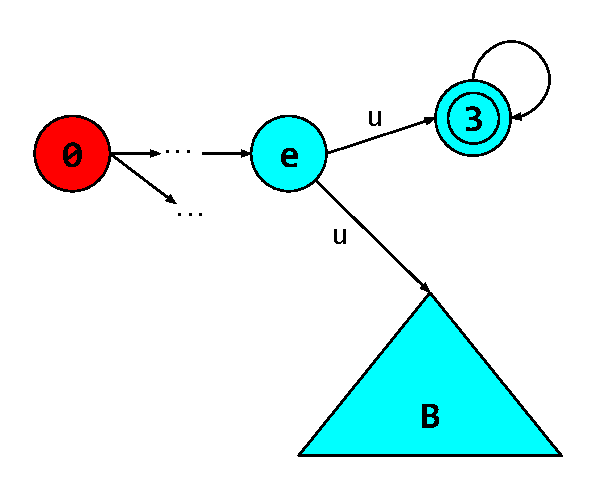
\includegraphics[width=\linewidth/2]{figures/FalenciasErrores.pdf}
 \caption{Caso no controlable que anteriormente propagaba Goal}
 \label{fig:falenciasErrores}
\end{figure}

% PROPAGACION LOCAL
Por otro lado, al propagar tenía una mirada local, perdiendo información sobre lo que sucede dentro del conjunto. Es así que no podía reconocer casos donde, por ejemplo, hay un loop no controlable entre dos estados y uno de ellos va no controlablemente a un error. En este caso es obvio que todo debe ser error pero según la mirada local ambos tienen \textit{una forma de escapar del error}, el otro estado del conjunto. Para una aclaración visual ver la fugura \ref{fig:propagarError}.

Incluso habiendo reconocido $\Goals$, no se puede propagar la información sin mirar un conjunto de nodos a la vez, en la figura \ref{fig:propagarGoal} se puede ver un ejemplo de esto. Aunque tanto $1$ como $2$ llegan al estado marcado $3$, ninguno puede forzarlo. Por ser non-blocking esto no nos molestaría y debería ser controlable, pero si miramos localmente al propagar $Goal$ desde $3$, no sabemos dónde nos lleva la transición no controlable, y deberiamos suponer lo peor.

En conclusión, es difícil decidir dónde hacer el corte. Son muchos casos y no se puede, localmente, distinguirlos a todos. Por ende es necesario un algoritmo más inteligente, con una mirada global del conjunto a propagar.
\begin{figure}[htb]
	\centering
	\makebox[\linewidth][c]{%
	\begin{subfigure}[t]{.5\textwidth}
		\centering
		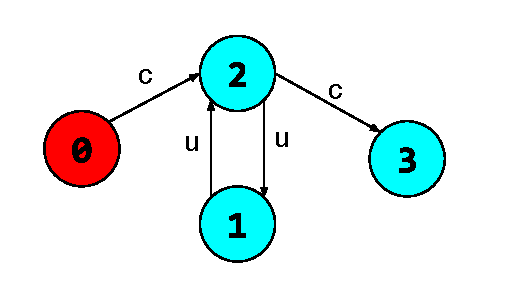
\includegraphics[width=\linewidth]{figures/PropagarError.pdf}  
		\caption{Propagar errores}
		\label{fig:propagarError}
	\end{subfigure}
	\begin{subfigure}[t]{.5\textwidth}
		\centering
		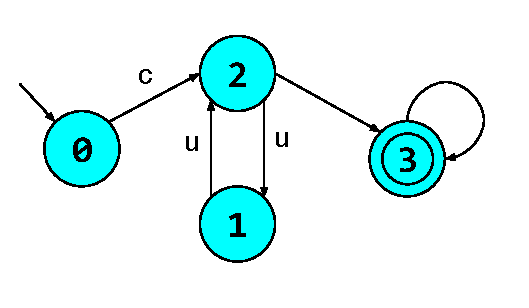
\includegraphics[width=\linewidth]{figures/PropagarGoal.pdf}  
		\caption{Propagar goals}
		\label{fig:propagarGoal}
	\end{subfigure}
	}
	\caption{Problemas de propagación local}
	\label{fig:propagacionLocal}
\end{figure}

% FALTA DE COMPLETITUD
Respecto a la falta de completitud, queda claro que teniendo una conclusión para cada uno de los estados hijos del inicial podemos definir si el problema es o no controlable. Lo que sucedía era que al tener conclusiones erroneas y problemas de propagación había ciertos casos donde, según el algoritmo de exploración el problema era controlable pero al llegar al constructor del controlador se daba cuenta que había estados a los cuáles les faltaba exploración y que, de hecho, tenían transiciones no controlables a estados sin mirar. Llegado ese punto devolvía que no había controlador, cuando de seguir explorando hubiese visto que lo que faltaba era algo ganador. Una ejemplo particular de esto puede verse en la figura \ref{fig:faltaCompletitud}, al terminar la exploración se concluyó que era controlable, sin embargo al querer construir el controlador se descubre que el estado $1$ tiene una no controlable por explorar, devolviendo entonces que no existe controlador.
\begin{figure}[htb]
 \centering
 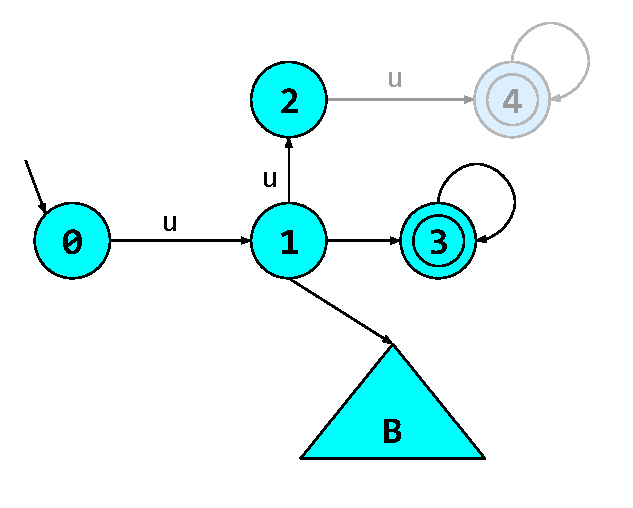
\includegraphics[width=\linewidth/2]{figures/faltaDeCompletitud.pdf}
 \caption{Ejemplo de falta de completitud, los estados en gris son los faltantes por explorar.}
 \label{fig:faltaCompletitud}
\end{figure}


%TODO EXPLICAR QUE NUESTRO ALGORITMO ES AGNÓSTICO A LA HEURÍSICA (COMO DEBERÍA), y algo que enganche este final con el comienzo del prox capitulo
    

